%%%%%%%%%%%%%%%%%%%%%%%% 
%
%   	   Total Variation Image Inpainting
%
%%%%%%%%%%%%%%%%%%%%%%%%
%
\documentclass[11pt,reqno,twoside]{amsart}
%
\synctex=1
%
%%%%%%%%%%%%%%%%%%%%%%
%
% 			Packages
%
%%%%%%%%%%%%%%%%%%%%%%
%
\usepackage{amscd}
\usepackage{amsfonts}
\usepackage{amsmath}
\usepackage{amssymb}
\usepackage{amsthm}
\usepackage{fancyhdr}
\usepackage{latexsym}
\usepackage[colorlinks=true, pdfstartview=FitV, linkcolor=blue, citecolor=blue, urlcolor=blue]{hyperref}
\usepackage{enumitem}      
\usepackage{mathtools}            
\usepackage{upgreek}
\usepackage{caption} 
\usepackage{indentfirst} % for indentation after chapter, section, subsection, etc.        
\usepackage{schemata} % for brackets around paragraphs
\usepackage{blindtext, rotating}   
\usepackage{soul} % for striking through text
\usepackage{graphicx} 
\usepackage{float}
\setstcolor{red}
%
\usepackage{color}
\usepackage{tikz}
\usetikzlibrary{arrows.meta}
\usetikzlibrary{decorations.markings}
\tikzset{->-/.style={decoration={
  markings,
  mark=at position #1 with {\arrow{>}}},postaction={decorate}}}
  \tikzset{middlearrow/.style={
        decoration={markings,
            mark= at position 0.55 with {\arrow{#1}} ,
        },
        postaction={decorate}
    }
}          
%
%%%%%%%%%%%%%%%%%%%%%%
%
% 		     New Commands
%
%%%%%%%%%%%%%%%%%%%%%%
%
\newcommand{\eee}[1]{\begin{equation}#1\end{equation}}
\newcommand{\sss}[1]{\begin{subequations}#1\end{subequations}}
\newcommand{\ddd}[1]{\begin{alignat}{2}#1\end{alignat}}
\newcommand{\mmm}[1]{\left(\begin{array}{ll}#1\end{array}\right)}
\newcommand{\nn}{\nonumber}
\newcommand{\p}{\partial}
\renewcommand{\c}{\mathcolor}
\definecolor{ddgreen}{RGB}{0,170,0}
\newcommand{\g}{\mathcolor{ddgreen}}
\renewcommand{\r}{\mathcolor{red}}
\renewcommand{\b}{\mathcolor{blue}}
\newcommand{\gtext}{\textcolor{ddgreen}}
\newcommand{\rtext}{\textcolor{red}}
\newcommand{\btext}{\textcolor{blue}}
\newcommand{\no}[1]{\left\| #1 \right\|}
\newcommand{\abs}[1]{\left| #1 \right|}
\newcommand{\supp}{\text{supp}}
%
% Hats Commands
%
\newcommand{\what}{\widehat}
\usepackage{scalerel,stackengine}
\stackMath
\newcommand\wwhat[1]{
\savestack{\tmpbox}{\stretchto{
  \scaleto{
    \scalerel*[\widthof{\ensuremath{#1}}]{\kern-.6pt\bigwedge\kern-.6pt}
    {\rule[-\textheight/2]{1ex}{\textheight}}
  }{\textheight} 
}{0.5ex}}
\stackon[1pt]{#1}{\tmpbox}
}
%
% Subsection and Subsubsection Definition
%
\makeatletter
\renewcommand\subsection{\@startsection{subsection}{2}%
  \z@{-0.8\linespacing\@plus-0.7\linespacing}{0.7\linespacing}%
  {\normalfont\bfseries}}
% \renewcommand\subsubsection{\@startsection{subsubsection}{3}%
%   \z@{-0.8\linespacing\@plus-0.7\linespacing}{0.7\linespacing}%
%   {\normalfont\itshape}}
% \makeatother
%
%%%%%%%%%%%%%%%%%%%%%%
%
% 	    For Math Mode Coloring
%
%%%%%%%%%%%%%%%%%%%%%%
%
\makeatletter
\def\mathcolor#1#{\@mathcolor{#1}}
\def\@mathcolor#1#2#3{%
\protect\leavevmode
\begingroup
\color#1{#2}#3%
\endgroup
}
\makeatother
%
%%%%%%%%%%%%%%%%%%%%%%
%
% 	           New Environments
%
%%%%%%%%%%%%%%%%%%%%%%
%
\theoremstyle{plain} 
\newtheorem{theorem}{Theorem}[section]
\newtheorem{proposition}{Proposition}[section]
\newtheorem{lemma}{Lemma}[section]
\newtheorem{corollary}{Corollary}[section]
\newtheorem{conjecture}{Conjecture}[section]
%
\theoremstyle{definition}
\newtheorem{definition}{Definition}[section]
\newtheorem{remark}{Remark}[section]
%
\newenvironment{Proof}[1][\proofname]
{\proof[\textnormal{\textbf{#1.}}]}{\endproof}
%
\renewcommand{\qedsymbol}{$\blacksquare$}
\renewcommand{\Re}{\operatorname{Re}}
\renewcommand{\Im}{\operatorname{Im}}
\newcommand{\argmin}{\operatorname{argmin}}
\newcommand{\argmax}{\operatorname{argmax}}
%

\def\Xint#1{\mathchoice
   {\XXint\displaystyle\textstyle{#1}}%
   {\XXint\textstyle\scriptstyle{#1}}%
   {\XXint\scriptstyle\scriptscriptstyle{#1}}%
   {\XXint\scriptscriptstyle\scriptscriptstyle{#1}}%
   \!\int}
\def\XXint#1#2#3{{\setbox0=\hbox{$#1{#2#3}{\int}$}
     \vcenter{\hbox{$#2#3$}}\kern-.5\wd0}}
\def\ddashint{\Xint=}
\def\dashint{\Xint-}

%%%%%%%%%%%%%%%%%%%%%%
%
%			Math Sizes
%
%%%%%%%%%%%%%%%%%%%%%%
%
\DeclareMathSizes{12}{12}{7}{5}
%Format: \DeclareMathSizes {t-size} {mt-size} {s-size} {ss-size}
%
%%%%%%%%%%%%%%%%%%%%%%
%
% 	   Coloring of Equations/Boxes
%
%%%%%%%%%%%%%%%%%%%%%%
%
\usepackage[framemethod=TikZ]{mdframed}
%
% Green Box
%
\newcommand{\fg}[1]
{
\begin{mdframed}
%
[  middlelinecolor=black, % border line color
   middlelinewidth=0pt, % border line thickness
   backgroundcolor=green!23, % background color - choose degree of  transparency
   roundcorner=10pt % corner rounding - 0 gives 90 degrees
 ] 
#1\end{mdframed}
}
%
% Cyan Box
%
\newcommand{\fc}[1]
{
\begin{mdframed}
%
[  middlelinecolor=black, % border line color
   middlelinewidth=0pt, % border line thickness
   backgroundcolor=cyan!23, % background color - choose degree of  transparency
   roundcorner=10pt % corner rounding - 0 gives 90 degrees
 ] 
#1\end{mdframed}
}
%
% Orange Box
%
\newcommand{\fo}[1]
{
\begin{mdframed}
%
[  middlelinecolor=black, % border line color
   middlelinewidth=0pt, % border line thickness
   backgroundcolor=orange!30, % background color - choose degree of  transparency
   roundcorner=10pt % corner rounding - 0 gives 90 degrees
 ] 
#1\end{mdframed}
}
%
% ANOTHER WAY for coloring boxes, that works for theorems too.
%
\usepackage[breakable, theorems, skins]{tcolorbox}
\tcbset{enhanced}
\DeclareRobustCommand{\cbox}[2][gray!20]{%
\begin{tcolorbox}[   %% Adjust the following parameters at will.
        %breakable,
        enhanced,
        left=10pt,
        right=10pt,
        top=10pt,
        bottom=10pt,
        colback=#1,
        colframe=#1,
        width=\textwidth, 
        enlarge left by=0mm,
        boxsep=0pt,
        arc=5pt,outer arc=5pt,
        colframe=black,
        boxrule=.6pt
        ]
        #2
\end{tcolorbox}
}
%

%%%%%%%%%%SUPPRESS WARNINGS
\hbadness=99999
\hfuzz=999pt
%%%%%%%%%%%%%%%%%%%%%%%%%%%%

\DeclareRobustCommand{\ccbox}[2][gray!20]{%
\begin{tcolorbox}[   %% Adjust the following parameters at will.
        %breakable,
        enhanced,
        left=10pt,
        right=10pt,
        top=10pt,
        bottom=10pt,
        colback=#1,
        colframe=#1,
        width=\textwidth, 
        enlarge left by=0mm,
        boxsep=0pt,
        arc=5pt,outer arc=5pt,
        colframe=black,
        boxrule=-1pt
        ]
        #2
\end{tcolorbox}
}

%
%%%%%%%%%%%%%%%%%%%%%%
%
% Numbering of Equations, Theorems, etc.
%
%%%%%%%%%%%%%%%%%%%%%%
%
\numberwithin{figure}{section}
\numberwithin{equation}{section}
%
%%%%%%%%%%%%%%%%%%%%%%%%%%%%%%
%
%  Page Setup (Margins, page numbering, headlines etc.)
%
%%%%%%%%%%%%%%%%%%%%%%%%%%%%%%
%
\usepackage{geometry}
\geometry{
  paper = letterpaper,
  top=1.16in, left=1in, right=1in, bottom=0.85in,
  footskip = 30 pt
}
\renewcommand{\baselinestretch}{1.1}
%
%%%%%%%%%%%%%%%%%%%%%%
%
%		   Table of Contents
%
%%%%%%%%%%%%%%%%%%%%%%
%
\makeatletter
\def\l@section{\@tocline{1}{0pt}{1pc}{}{}}
\def\l@subsection{\@tocline{2}{0pt}{1pc}{4.6em}{}}
\def\l@subsubsection{\@tocline{3}{0pt}{1pc}{7.6em}{}}
% \renewcommand{\tocsection}[3]{%
%   \indentlabel{\@ifnotempty{#2}{\makebox[2.3em][l]{%
%     \ignorespaces#1 #2.\hfill}}}#3}
\renewcommand{\tocsubsection}[3]{%
  \indentlabel{\@ifnotempty{#2}{\hspace*{2.3em}\makebox[2.3em][l]{%
    \ignorespaces#1 #2.\hfill}}}#3}
\renewcommand{\tocsubsubsection}[3]{%
  \indentlabel{\@ifnotempty{#2}{\hspace*{4.6em}\makebox[3em][l]{%
    \ignorespaces#1 #2.\hfill}}}#3}
\makeatother 
\setcounter{tocdepth}{4}
%
% Equation Conditions 
%
\usepackage{array,tabularx}
\newenvironment{conditions*}
  {\par\vspace{\abovedisplayskip}\noindent
   \tabularx{\columnwidth}{>{$}l<{$} @{\ : } >{\raggedright\arraybackslash}X}}
  {\endtabularx\par\vspace{\belowdisplayskip}}
\setlength\parindent{15pt}
%
\newtheorem{problem}{Problem}
\usepackage{mathrsfs}
%
% Meta Data
%
\begin{document}

\title{AMATH 515 - Optimization \\ Total Variation Image Inpainting Using Split Bregman \\ March 8, 2024}
\author{Catherine Johnston}

%\vspace*{-1.55cm}
\maketitle
%\vspace*{-0.4cm}

\markboth{Total Variation Image Inpainting}{Catherine Johnston}

\section{Motivation}

If a provided digital image is missing pixels in a region, image inpainting is the process of approximating the missing region using the data from the known pixels.  A complete image can also have pixels removed in an undesired region and then replaced via inpainting. There are various methods of image inpainting, and the two in particular that we wish to consider in this project are Laplace's equation inpainting ($H^1$ inpainting) and total variation (TV) inpainting (specifically the split Bregman algorithm), which will both be described in detail in the following sections and then implemented in code to consider various applications.  The efficiency (runtime) and accuracy of each method will then be compared.  Some example applications of image inpainting are as follows:
\begin{itemize}
\item[(a)] Filling in missing sections of an incomplete image.
\item[(b)] Removing an undesirable feature from an image, such as a stain on cloth. 
\item[(c)] Editing a hiking trail map with intersecting trails to remove a trail that has been shut down due to a safety hazard while maintaining continuity of the other trails on the map.
\end{itemize}
Applications (b) and (c) will be implemented in this project using sample images from the public domain.  To simplify the model and its implementation, we consider greyscale images rather than color images.

\newpage 

\section{Laplace's Equation Inpainting}

A classical approach to inpainting is to apply Laplace's equation in a process also sometimes called $H^1$ inpainting, which is presented in \cite{ge2012}.  Consider a greyscale image $g: \Omega \to \mathbb{R}$, where each $x \in \Omega$ is a (infinitesimally small) pixel in the image and each $g(x) \in \mathbb{R}$ represents the shade of grey of that (infinitesimally small) pixel.  This model will of course need to be discretized to be implemented in code.  We perform inpainting of an open set of pixels $D \subsetneq \Omega$, not necessarily connected.  

Laplace's equation is given by $\Delta u(x) = 0$, where $\Delta = \nabla^2$ is the Laplacian operator.  Assuming $g(x) = u(x)$ for all $x \in \Omega \setminus D$, we seek a solution to the Laplace's equation boundary value problem given by
\begin{equation*}
\begin{cases}
0= \Delta u(x), & x \in D, \\ 
g(x) = u(x), & x \in \partial D,
\end{cases}
\end{equation*}
which can be solved for $u(x)$ to determine the inpainted image $u: \Omega \to \mathbb{R}$.  The resulting image as defined above will exactly match the original image $g: \Omega \to \mathbb{R}$ outside the inpainted region $D$ and will approximate the original image inside the inpainted region.

The name ``$H^1$ inpainting'' comes from the use of the $H^1$-seminorm of $u(x)$ over $D$ given by
\begin{equation*}
\|u\|_{H^1(D)}^2 \doteq \int_D |\nabla u(x)|^2 dx,
\end{equation*}
which is also the $L^2$-norm of $\nabla u(x)$ over $D$.  A function $u(x) \in H^1(D)$ if $\|u\|_{H^1(D)} < \infty$.  Observe also that $H^1(D) = W^{1,2}(D)$, a Sobolev space of $L^2$ functions over $D$.  Furthermore, recall Dirichlet's principle that a Laplace's equation inpainting solution in $C^2(D)$ (the set of twice-continuously differentiable functions defined on $D$) has minimal $H^1$-seminorm over $D$ across all functions in $C^2(D)$ satisfying the boundary condition, a result stated in \cite{ev1998}.  The proof of this fact is derived from Green's identity.

\newpage 

\section{Total Variation Inpainting}

A more computationally effective method of image inpainting is total variation (TV) inpainting, which is also presented in \cite{ge2012}.  Instead of the $H^1$-seminorm, we use the total variation seminorm of $u(x)$ over $\Omega$, given by
\begin{equation*}
\|u\|_{\text{TV}(\Omega)} \doteq \int_\Omega |Du(x)| = \operatorname{sup}\left\{\int_\Omega u(x) (\nabla \cdot f(x))dx: \,\, f(x) \in C_c^1(\Omega, \mathbb{R}^2)^2, \, \|f\|_2 \leqslant 1 \right\},
\end{equation*}
where $C_c^1(\Omega, \mathbb{R}^2)^2$ is the Cartesian product of two spaces of compactly supported continuously differentiable functions from $\Omega$ to $\mathbb{R}^2$.  For smooth $u(x)$, the total variation seminorm can be written as 
\begin{equation*}
\|u\|_{\text{TV}(\Omega)} = \int_\Omega |Du(x)| = \int_\Omega |\nabla u(x)|dx,
\end{equation*}
where $u: \Omega \to \mathbb{R}$ is again the inpainted image.  Furthermore, instead of $H^1(D)$, we consider the space of functions of bounded variation (BV) over $\Omega$, where $u(x)$ is in $\text{BV}(\Omega)$ if there exists some Radon measure $Du(x)$ where
\begin{equation*}
\int_\Omega u(x) (\nabla \cdot f(x)) dx = -\int_\Omega \langle f(x), Du(x) \rangle
\end{equation*}
for all $f(x) \in C_c^1(\Omega, \mathbb{R}^2)^2$.  

To perform total variation inpainting, we seek the function of bounded variation $u(x) \in \text{BV}(\Omega)$ solving the optimization problem
\begin{equation*}
\argmin_{u(x) \in \text{BV}(\Omega)} \left[  \|u\|_{\text{TV}(\Omega)} + \frac{\lambda}{2} \int_{\Omega \setminus D} (g(x) - u(x))^2 dx\right]
\end{equation*}
for fixed $\lambda > 0$, where we still define open set $D \subsetneq \Omega$.  Thus, given original image $g: \Omega \to \mathbb{R}$, we obtain the inpainted image $u: \Omega \to \mathbb{R}$, which will exactly match the original image outside the inpainted region $D$ and will approximate the original image inside the inpainted region.

\newpage 

\section{Implementation}

In this project, total variation image inpainting will be implemented using the split Bregman approach presented in \cite{ge2012}.  Total variation image inpainting can also be implemented using other algorithms, such as the ADMM algorithm presented in \cite{qgm2014}.  The split Bregman algorithm itself was developed by Goldstein and Osher in \cite{go2009}.

After discretizing each dimension of the image $g: \Omega \to \mathbb{R}$ into the $N$-vector $(g_0, \cdots, g_{N-1})$, we define its discrete derivative as the forward difference
\begin{equation*}
\partial g = \begin{pmatrix} \partial g_0 \\ \vdots \\ \partial g_{N-2} \\ \partial g_{N-1} \end{pmatrix} = \begin{pmatrix} -1 & 1 & \cdots & 0 & 0 \\ \vdots & \ddots & \ddots & \ddots & \vdots \\ 0 & 0 & \cdots & -1 & 1 \\ 0 & 0 & \cdots & 0 & 0 \end{pmatrix}\begin{pmatrix} g_0 \\ \vdots \\ g_{N-2} \\ g_{N-1} \end{pmatrix}.
\end{equation*}
Since we are working in the two dimensional space $C_c^1(\Omega, \mathbb{R}^2)^2$, we define $\partial_x$ and $\partial_y$ as the discrete derivatives along the dimensions $x$ and $y$, respectively.  Thus, we define the discrete gradient as $\nabla \doteq (\partial_x,\partial_y)^T$.  Similarly, we define the discrete divergence $\nabla \cdot \doteq -\nabla^* = -\partial_x^* - \partial_y^*$ and the discrete Laplacian $\Delta \doteq \nabla \cdot \nabla$, where $\cdot^*$ is the adjoint.  More particularly, in the image interior, we have the formulas
\begin{align*}
\begin{cases}
\nabla \cdot u = u_{ij}^x - u_{(i-1)j}^x + u_{ij}^y - u_{i(j-1)}^y, \\ 
\Delta u = -4u_{ij} + u_{(i+1)j} + u_{(i-1)j} + u_{i(j+1)} + u_{i(j-1)},
\end{cases}
\end{align*}
as discussed in \cite{ge2012b}.  Finally, we discretize the total variation seminorm as 
\begin{equation*}
\|u\|_{\text{TV}(\Omega)} \approx \sum_{i=0}^{N-1} \sum_{j=0}^{N-1} |\nabla u_{ij}|.
\end{equation*}

To implement Laplace's equation inpainting, we set $u_{ij} = g_{ij}$ for each pixel outside the region $D$ and then perform Gauss-Seidel iterations
\begin{align*}
G_{ij} = \frac{1}{4}\Big[u_{(i+1)j} + u_{(i-1)j} + u_{i(j+1)} + u_{i(j-1)}\Big]
\end{align*}
away from the boundary, where we then set $u_{ij} = G_{ij}$ for each pixel in the region $D$.  The region $D$ is constructed using an indicator function of all sufficiently white or black pixels.  Boundary pixels must be handled case by case, where a more detailed implementation can be seen in our code.  We continue to iterate this process until 
\begin{equation*}
\|u - u_{\text{prev}}\|_2 < \varepsilon
\end{equation*}
for error tolerance $\varepsilon = \|g\|_2 \times 10^{-5}$ as chosen in \cite{ge2012}.

The split Bregman algorithm for total variation image inpainting solves the constrained optimization problem
\begin{equation*}
\begin{cases}
\argmin_{d,u} \sum_{i=0}^{N-1} \sum_{j=0}^{N-1} |d_{ij}| + \frac{1}{2}\sum_{i=0}^{N-1} \sum_{j=0}^{N-1} \lambda_{ij} (g_{ij} - u_{ij})^2, \\
d = \nabla u.
\end{cases}
\end{equation*}
where $\lambda$ is a pixel-varying parameter chosen to ease computation.  Each iteration solves the subproblem
\begin{equation*}
\argmin_{d,u} \sum_{i=0}^{N-1} \sum_{j=0}^{N-1} |d_{ij}| + \frac{1}{2}\sum_{i=0}^{N-1} \sum_{j=0}^{N-1} \lambda_{ij} (g_{ij} - u_{ij})^2 + \frac{\gamma}{2}\sum_{i=0}^{N-1} \sum_{j=0}^{N-1} |d_{ij}-\nabla u_{ij} - b_{ij}|^2
\end{equation*}
for variable $b$ and some parameter $\gamma > 0$, generally a moderate value to ensure fast convergence.  We choose $\gamma = 5$ as in \cite{ge2012}.  This is implemented by alternating between minimizing over $d$ and $u$ for constant $u$ or $d$, respectively, which is called an alternating direction method.  

Since the second term does not depend on $d$, we minimize over $d$ by solving the optimization problem
\begin{equation*}
\argmin_{d} \sum_{i=0}^{N-1} \sum_{j=0}^{N-1} |d_{ij}|+\frac{\gamma}{2}\sum_{i=0}^{N-1} \sum_{j=0}^{N-1} |d_{ij}-\nabla u_{ij} - b_{ij}|^2
\end{equation*}
for constant $u$, which has solution
\begin{equation*}
d_{ij} = \frac{\nabla u_{ij} + b_{ij}}{|\nabla u_{ij} + b_{ij}|} \max\left\{|\nabla u_{ij} + b_{ij}|-\frac{1}{\gamma}, 0\right\},
\end{equation*}
as provided in \cite{ge2012b}.  Similarly, since the third term does not depend on $u$, we minimize over $u$ by solving the optimization problem
\begin{equation*}
\argmin_{u} \sum_{i=0}^{N-1} \sum_{j=0}^{N-1} \lambda_{ij} (g_{ij} - u_{ij})^2 + \gamma\sum_{i=0}^{N-1} \sum_{j=0}^{N-1} |d_{ij}-\nabla u_{ij} - b_{ij}|^2
\end{equation*}
for constant $d$, which yields the solution to the equation
\begin{equation*}
\lambda u - \gamma \Delta u = \lambda g - \gamma \nabla \cdot (d-b),
\end{equation*}
which can be approximately solved using one iteration of Gauss-Seidel per iteration of split Bregman. From \cite{go2009}, we know that (away from the boundary) the solution to the $u$-subproblem is given by
\begin{align*}
G_{ij} &= \frac{\gamma}{\lambda+4\gamma}\Big[u_{(i+1)j} + u_{(i-1)j} + u_{i(j+1)} + u_{i(j-1)} + d_{(i-1)j}^x - d_{ij}^x + d_{i(j-1)}^y - d_{ij}^y \nn\\ &\quad- b_{(i-1)j}^x + b_{ij}^x - b_{i(j-1)}^y + b_{ij}^y \Big] + \frac{\lambda}{\lambda+4\gamma}g_{ij},
\end{align*}
where we then set $u_{ij} = G_{ij}$.  Finally, before entering the next iteration, we update $b \mapsto b+\nabla u - d$.  We iterate the algorithm until we reach \begin{equation*}
\|u - u_{\text{prev}}\|_2 < \varepsilon
\end{equation*}
for error tolerance $\varepsilon = \|g\|_2 \times 10^{-5}$ as chosen in \cite{ge2012}.

\newpage 

\section{Results}

Both Laplace's equation inpainting and total variation inpainting were tested for the following public domain test images, greyscaled using our code:

\begin{center}
\begin{figure}[h]
\caption{An image of a stained strip of cloth, obtained from Creative Commons at \url{https://commons.wikimedia.org/wiki/File:Cloth_strips_with_blood_-_Public_Domain.jpg }.  Photographed by Lisa Redfern and uploaded in 2014.}
\vskip 1mm
\includegraphics[width = 8cm]{Original Stain}
\end{figure}
\end{center}
\begin{center}
\begin{figure}[h]
\caption{A cropped version of an image of a 1952 map of Emigrant Trail from P.M. Weddell, obtained from flickr Creative Commons at \url{https://www.flickr.com/photos/188645737@N03/}. Uploaded by the Donner Summit Historical Society in 2020.}
\vskip 1mm
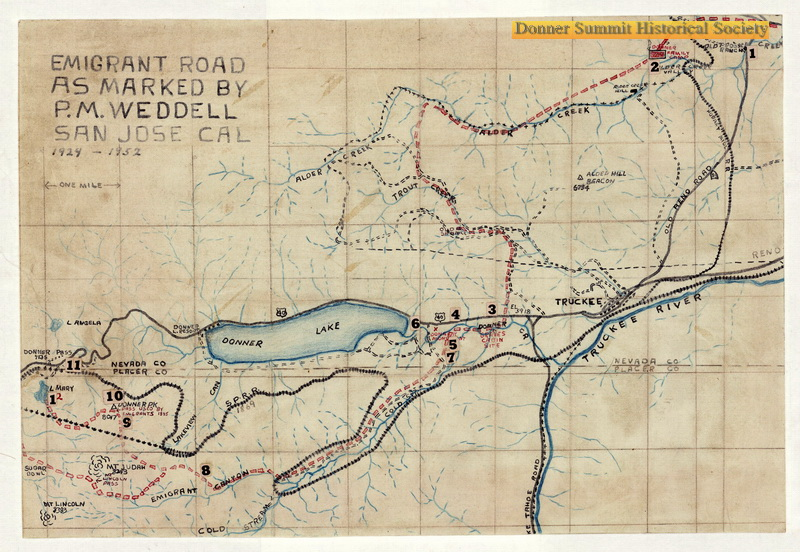
\includegraphics[width = 8cm]{Original Map}
\end{figure}
\end{center}

\newpage

In order to remove the stains from the image of the cloth strips, the image in Figure 5.1 was inpainted in the regions marked below.  Similarly, in order to remove a trail from the map of Emigrant Trail, the image in Figure 5.2 was inpainted in the region marked below.  Both images are presented below with the inpainted regions marked black and white, respectively:

\begin{center}
\begin{figure}[h]
\caption{Figure 5.1 but with the inpainted regions marked black.}
\vskip 1mm
\includegraphics[width = 8cm]{Incomplete Stain}
\end{figure}
\end{center}
\begin{center}
\begin{figure}[h]
\caption{Figure 5.2 but with the inpainted region marked white.}
\vskip 1mm
\includegraphics[width = 8cm]{Incomplete Map}
\end{figure}
\end{center}

\newpage

As the final step prior to implementation, the images were cropped into exact squares using the tool \url{https://squareanimage.com/}, with the versions of the images actually being implemented below:

\begin{center}
\begin{figure}[h]
\caption{The actually implemented image of the stained cloth, greyscaled and cropped to be square (168 $\times$ 168).}
\vskip 1mm
\includegraphics[width = 7cm]{Final Stain}
\end{figure}
\end{center}
\begin{center}
\begin{figure}[h]
\caption{The actually implemented image of the map of Emigrant Trail, greyscaled and cropped to be square (154 $\times$ 154).}
\vskip 1mm
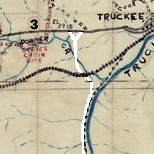
\includegraphics[width = 7cm]{Final Map}
\end{figure}
\end{center}

\newpage

Laplace's equation image inpainting yielded the following results, which were especially good for the image of the stained cloth strip:

\begin{center}
\begin{figure}[h]
\caption{The image of the stained cloth inpainted with Laplace's equation.  The stains have now been removed.  The runtime to generate this image was $19.241$ seconds, using 467 iterations.}
\vskip 1mm
\includegraphics[width = 7cm]{Final Stain H1}
\end{figure}
\end{center}
\begin{center}
\begin{figure}[h]
\caption{The image of the map of Emigrant Trail inpainted with Laplace's equation.  The trail has now been removed, albeit not as well as the cloth stains.  The runtime to generate this image was $1.622$ seconds, using 51 iterations.}
\vskip 1mm
\includegraphics[width = 7cm]{Final Map H1}
\end{figure}
\end{center}

\newpage

We encountered several difficulties when implementing total variation image inpainting using the split Bregman approach.  First, several details of how to adapt total variation denoising into inpainting were absent from \cite{ge2012}, the primary source for this project.  Second, the contribution of the solution of the $d$-subproblem canceled out the contribution of the Laplacian of $u$ when solving the $u$-subproblem using Gauss-Seidel, leading to no pixels being changed each iteration.  Regardless, the test images were ran with the same number of iterations to test and compare runtime, although likely the number of iterations would differ if total variation inpainting were implemented correctly.  In summary, total variation inpainting took $106.344$ seconds to run for the stained cloth and $9.465$ seconds to run for the trail map.  Around 6 times more time elapsed compared to Laplace's equation inpainting.  The code for this project can be found in the Jupyter notebook ``Project\_Catherine\_Johnston.ipynb'' and can be accessed using the Github repository \url{https://github.com/catherinemj/AMATH-515-Project}.

\newpage

\begin{thebibliography}{1000000}
%
\bibitem[Ev]{ev1998} Evans, L. Partial Differential Equations. \textit{Graduate Studies in Mathematics} \textbf{19}, American Mathematical Society, ISBN: 0821807722 (1998).
%
\bibitem[GeA]{ge2012b} Getreuer, P. Rudin-Osher-Fatemi Total Variation Denoising using Split Bregman. \textit{Image Processing On Line} \textbf{2}, 74-95 (2012).
%
\bibitem[GeB]{ge2012} Getreuer, P. Total Variation Inpainting using Split Bregman. \textit{Image Processing On Line} \textbf{2}, 147-157 (2012).
%
\bibitem[GO]{go2009} Goldstein, T. Osher, S. The Split Bregman Method for L1 Regularized Problems. \textit{SIAM Journal on Imaging Sciences} \textbf{2}, 323-343 (2009).
%
\bibitem[QGM]{qgm2014} Qin, Z. Goldfarb, D. Ma, S. An Alternating Direction Method for Total Variation Denoising. \textit{Optimization Methods and Software} \textbf{30}, 594-615 (2014).
%
\end{thebibliography}

\end{document}